\documentclass{vipweekly}
\usepackage[colorlinks, hyperfootnotes]{hyperref}
\usepackage{hhline}
\usepackage[noadjust]{cite}
\usepackage{listings}
\usepackage{lipsum}
\usepackage{amsfonts}
\usepackage{algorithm} % Pseudo code 작성용
\usepackage{algorithmicx} % Pseudo code 작성용
\usepackage{algpseudocode} % Pseudo code 작성용
\usepackage{xcolor}

\renewcommand{\citedash}{--}

\title{Weekly Report} %% Title은 Weekly Report로 고정합니다.
%% Grade는 아래와 같이 작성합니다. 
\grade{Master's Program} % For 석사과정
\grade{Combined Master's-Doctoral Program} % For 석박사통합과정
\grade{Doctoral Program} % For 박사과정
\grade{U-surf Program} % For 석사과정
\author{Dong-Wook Kim} % 이름은 영문으로 작성합니다. 
\date{\today} % Date는 작성 날짜로 고정합니다. 

\begin{document}
\maketitle
\hypersetup{citecolor=blue}

\section*{Milestones}
\begin{itemize} 
    \item U-surf Program \\
    \begin{itemize}
        \item U-surf Program Due: Jul. 28th\\
    \end{itemize}
\end{itemize}
이번 주에는 
\begin{enumerate}
    \item InfoNeRF\cite{Infonerf} 논문 리뷰
    \item custom data를 이용한 InfoNeRF학습
    % \begin{itemize}
    %     \item colmap 
    %     \item Backpropagation 구현
    % \end{itemize}
    
\end{enumerate} 
등을 진행하기로 했습니다.


\section{InfoNeRF\cite{Infonerf} 논문 리뷰}

Infonerf는 nerf모델의 추론과정을 4장의 이미지를 사용하여 추론하도록 하는 nerf에 entropy term과 
kl divergence loss term을 더해 few shot scene reconstruction이 가능하도록 해주는 모델이다.
저자들이 말하길 Infonerf는 기존 few shot nerf 와 다르게 uv map, 
depth map과 같은 추가적인 scene 정보가 필요하지 않고, 기존 nerf에서 
entropy term 과 kl divergence loss term만을 추가하면 되기 때문에 학습 속도 
저하 또한 없이 scene reconstruction이 가능하다고 설명한다.
그렇가면 앞서 말한 두가지 term이 기존 nerf에 어떠한 부분을 대체하는지 알아보자

\subsection{Ray entropy}

기존 nerf에 ray opacity에 Shannon Entropy(정보 엔트로피)를 더해준다.
Shannon Entropy는 불확실성이 클 수록 더욱 큰 수가 나온다. 
다시말해 물체에 가로막힌 point인지 그렇지 않은지가 불명확할 수록 큰 값이 나오게 된다. 
따라서 해당값이 $\epsilon$ 이하라면 그 이후 point 들은 학습하지 않는다. 
수식을 통해 그 의미를 알아보겠다.

\begin{equation}
    p\left(\mathrm{r}_i\right)=\frac{\alpha_i}{\sum_j \alpha_j}=\frac{1-\exp \left(-\sigma_i \delta_i\right)}{\sum_j 1-\exp \left(-\sigma_j \delta_j\right)}    \label{eq:nerf_continuous}
\end{equation}
먼저 $p\left(\mathrm{r}_i\right)$ 위와 같이 정의한다. 한 point에서의 투과도를 ray 상에 모든 투과도의 누적합으로 나눠준 결과이다.\\


\begin{equation}
    H(\mathbf{r})=-\sum_{i=1}^N p\left(\mathbf{r}_i\right) \log p\left(\mathbf{r}_i\right).
    \label{eq:nerf_continuous}
\end{equation}

$H(\mathbf{r})$는 Shannon entropy을 나타내는 식이다. 어떤한 사건에 발생 확률이 낮을수록 정보량이 더욱 크다. 


여기까지 정리하여 보면 투과도 즉 opacity값은 0\~1 사이의 값을 갖기 때문에 확률값이라 볼 수 있다. 
해당 지점에 투명도가 낮을 수록 정보량을 클것이고, 불투명한 부분일수록  정보량은 적을 것이다. 
따라서 해당 값이 작아 지도록 학습하면 적합한 point의 위치를 찾는데 도움을 줄 수 있다.\\


다만 ray 가 아무 물체도 hit 하지않는다면 p 식의 분모가 작아지기 때문에 낮은 정보량를 갖는다. 
따라서 아래와 같은 별도 과정을 추가해주어 물체를 지나는지 확인한다.

\begin{equation}
    Q(\mathrm{r})=\sum_{i=1}^N 1-\exp \left(-\sigma_i \delta_i\right)
\end{equation}

ray 상에 물체가 존재하는지 판단하기 위해 투과도에 누적합을 사용하며 이를  $Q(\mathrm{r})$로 정의한다.

\begin{equation}
    M(\mathrm{r})= \begin{cases}1 & \text { if } Q(\mathrm{r})>\epsilon \\ 0 & \text { otherwise }\end{cases}
\end{equation}

$Q(\mathrm{r})$을 통해 얻은 값이 $\epsilon$이하의 entropy의 누적합을 갖는다면 
물체를 지나는 ray가 아니라고 판단된다면 학습을 진행하지 않는다.

\begin{equation}
    \mathcal{L}_{\text {entropy }}=\frac{1}{\left|\mathcal{R}_s\right|+\left|\mathcal{R}_u\right|} \sum_{\mathbf{r} \in \mathcal{R}_s \cup \mathcal{R}_u} M(\mathrm{r}) \odot H(\mathrm{r})
\end{equation}

앞서 구한 함수들을 이용하여 위와 같은 loss function을 정의 한다

\subsection{KL divergence} 

마지막으로 ray entropy를 사용할 경우 few shot image에 overfitting되는 이슈가 있다고 한다.
따라서 약간의 불확실성을 주기 위해 kl divergence의 개념을 추가한다.
-5\~5 도 정도 벗어난 ray와 원본 ray를 이용하여 둘 사이 kl divergence를 최소화하는 loss term을 더해준다.
(두 분포 사이를 계산하는 수치)
즉, 기존 nerf 에 input으로 들어가던 $(\theta,\phi)$ 값을 +-5도 정도 조절하여 넣어준 것이다.

\begin{equation}
    \mathcal{L}_{\mathrm{KL}}=D_{\mathrm{KL}}(P(\mathrm{r}) \| P(\tilde{\mathrm{r}}))=\sum_{i=1}^N p\left(\mathrm{r}_i\right) \log \frac{p\left(\mathrm{r}_i\right)}{p\left(\tilde{\mathrm{r}}_i\right)}
\end{equation}

개인적인 해석을 한번 해보자면 약간의 데이터 증강 강제적으로 오차를 주는 과정 진행하여
overfitting을 해결한것 같다. 
비슷한 시도를 머신러닝 알고리즘에서 본것이 있던것 같다. 
해당 방법이 좋은 방법이라고 생각되지는 않지만,
nerf에 경우 positional encoding을 거치기 때문에 저러한 variation 주어도 학습결과를
망치지 않고 overfitting을 방지하는게 아닐까 생각한다.

\begin{equation}
    \mathcal{L}_{\text {total }}=\mathcal{L}_{\text {RGB }}+\lambda_1 \mathcal{L}_{\text {entropy }}+\lambda_2 \mathcal{L}_{\mathrm{KL}}
\end{equation}

앞서 설명한 각정 loss function을 이용하여 최종적인 loss function을 정의한다.
각 loss 대한 weighted sum 을 진행한다. 


정말 간단하지만 위 내용이 Infonerf에 전부이다. 아이디어는 간단하지만 내용은 수학적인 내용이 많아 쉽지만은 않다.

loss function을 잘 설계한 것 많으로 이전 모델을 상당히 개선한 모습이 인상적이다. 
아직 공부가 부족해 Infonerf에 방법이 이후 nerf 모델에 항상 성능향상을 위해 사용되는지는 모르겠지만, 실제 코드를 돌려본 결과 custom dataset에 대해 각종 파라미터에 매우 민감한 것 같았다.

\newpage

\section{Custom data를 이용한 InfoNeRF 학습}

\subsection{실험 데이터} 


\begin{figure}[h]
    \centering

    \subfloat[colmap]{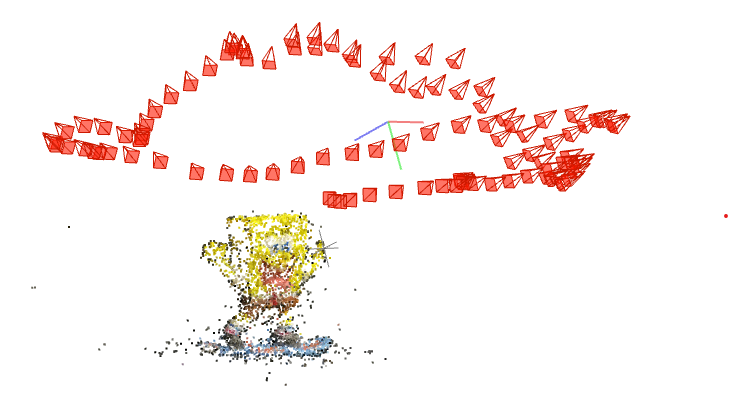
\includegraphics[width=0.7\textwidth]{../images/230717/colmap.png}}\hfill\\

    \subfloat[spongebobGT1]{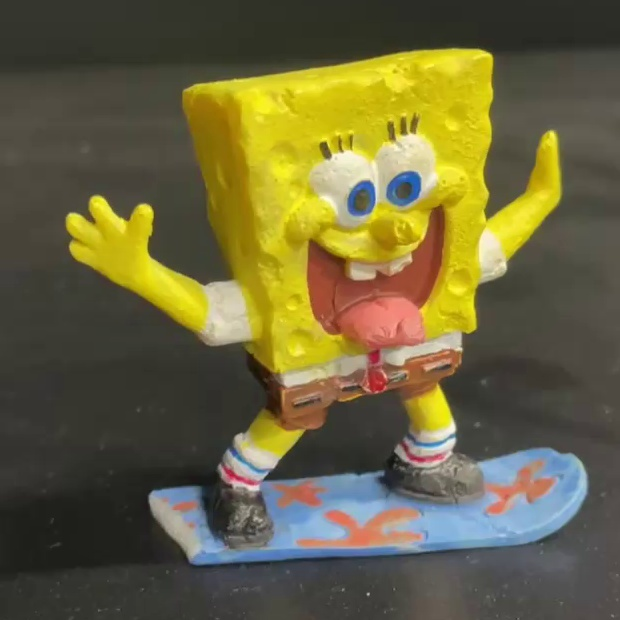
\includegraphics[width=0.3\textwidth]{../images/230717/spongebobGT1.png}}\hfill
    \subfloat[spongebobGT2]{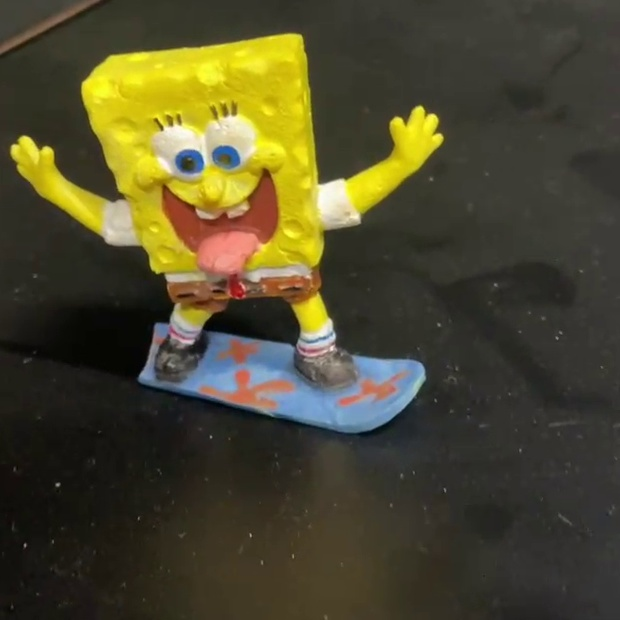
\includegraphics[width=0.3\textwidth]{../images/230717/spongebobGT2.png}}\hfill
    \subfloat[spongebobGT3]{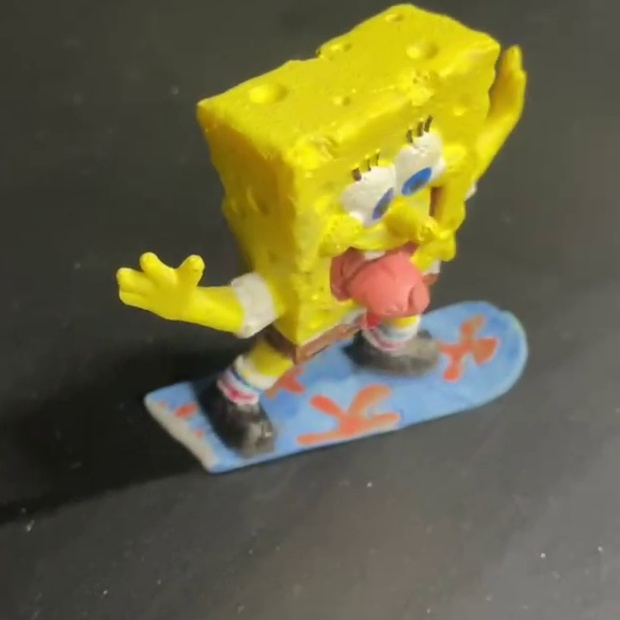
\includegraphics[width=0.3\textwidth]{../images/230717/spongebobGT3.png}}\hfill

    \caption{Custom data for InfoNeRF}
    \label{fig:dataset}
\end{figure}


아이폰을 이용한 촬영한 스폰지밥 영상 활용, 
배경 제거 최대한 동일한 거리에서 데이터 수집하였다.

\subsection{실험 결과}

예상보다 좋지않은 성능의 결과를 얻을 수 있었다. 
\newpage

\begin{figure}[h]
    \centering
    \subfloat[view1 rendered image]{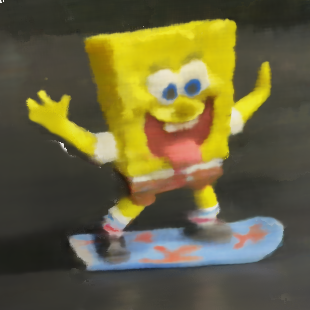
\includegraphics[width=0.3\textwidth]{../images/230717/000_018.png}}\hfill
    \subfloat[view2 rendered image]{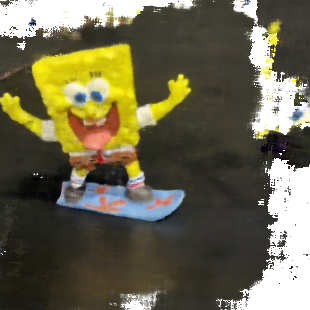
\includegraphics[width=0.3\textwidth]{../images/230717/078_018.png}}\hfill
    \subfloat[view3 rendered image]{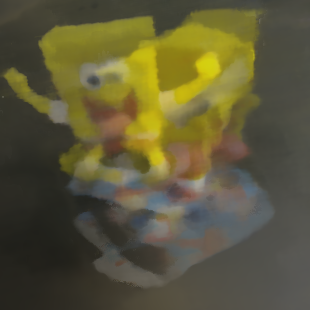
\includegraphics[width=0.3\textwidth]{../images/230717/003_018.png}}\hfill

    \subfloat[view1 depthmap]{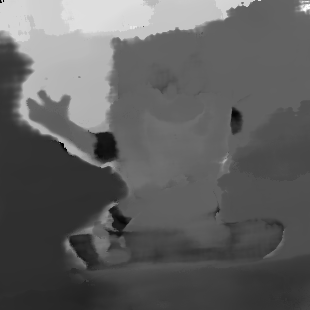
\includegraphics[width=0.3\textwidth]{../images/230717/000_depth_018.png}}\hfill
    \subfloat[view2 depthmap]{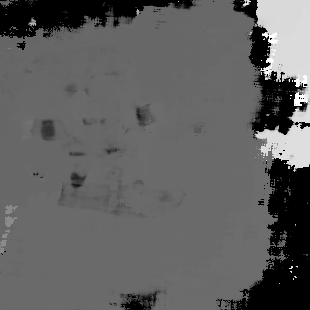
\includegraphics[width=0.3\textwidth]{../images/230717/078_depth_018.png}}\hfill
    \subfloat[view3 depthmap]{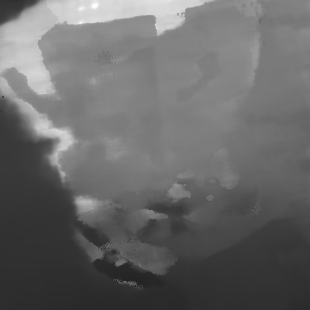
\includegraphics[width=0.3\textwidth]{../images/230717/003_depth_018.png}}\hfill

    \caption{InfoNeRF Results}
    \label{fig:Results}
\end{figure}

특정 view에서는 굉장히 그럴듯한 모습을 보이지만 input data로 제공된 view에 overfitting된 모습을 확인가능하다. depthmap
또한 물체에 형상을 배경과 분리하여 완벽히 추론하였다고 볼 수 없는 결과가 나왔다.

\begin{figure}[h]
    \centering

    \subfloat{\includegraphics[width=0.9\textwidth]{../images/230717/Infonerf.png}}\hfill\\
    \caption{InfoNeRF DTU dataset}
    \label{fig:Infonerf}
\end{figure}

\newpage

예상되는 원인은 다음과 같다.
\begin{enumerate}
    \item camera extrinsic의 일부가 잘못되었다.
    \item InfoNeRF의 한계이다. 
    \begin{enumerate}
        \item \ref{fig:Infonerf}의 결과를 보면 depth map이 대략적인 형상만을 보여줄 뿐 완벽한 결과를 보여주지는 못하고 있다.
        \item 좋은 결과가 나왔던 lego dataset에 경우 배경이 없지만 custom data에는 배경이 존재한다.
    \end{enumerate}
\end{enumerate}


\subsection{추가 실험}

\begin{figure}[h]
    \centering
    \subfloat{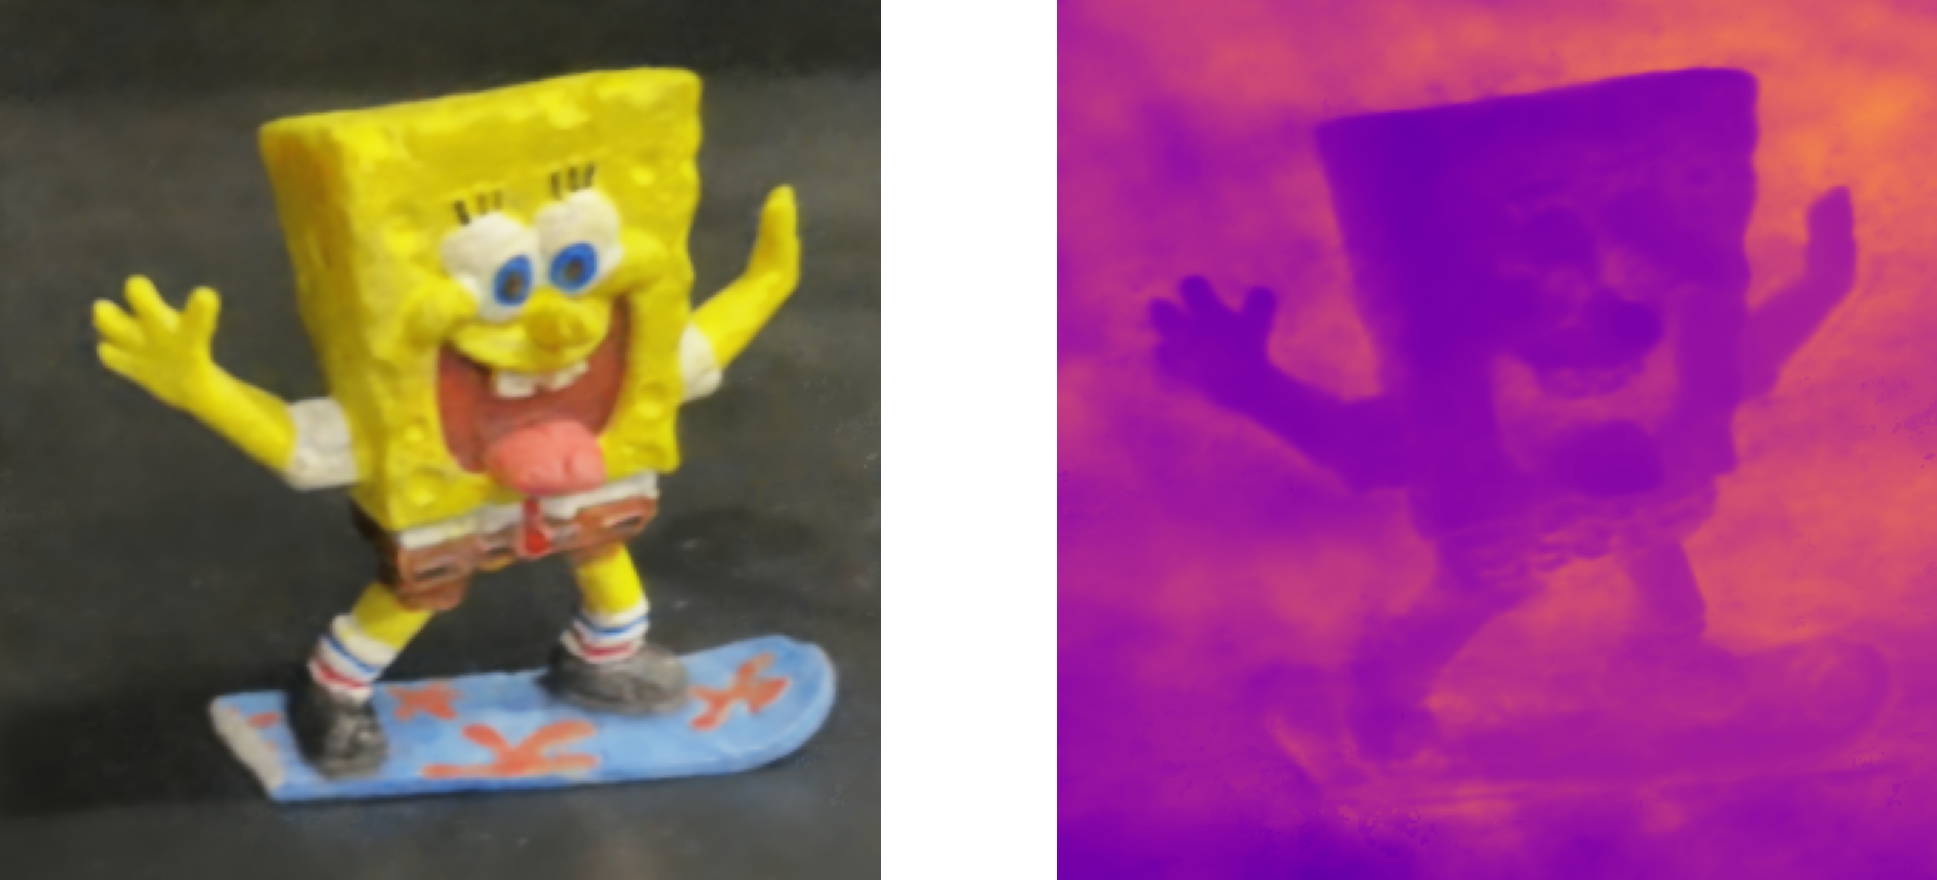
\includegraphics[width=0.5\textwidth]{../images/230717/hash_nerf.png}}\hfill\\
    \caption{hash nerf with same setting}
    \label{fig:Infonerf}
\end{figure}

\begin{figure}[h]
    \centering
    \subfloat[view1 rendered image]{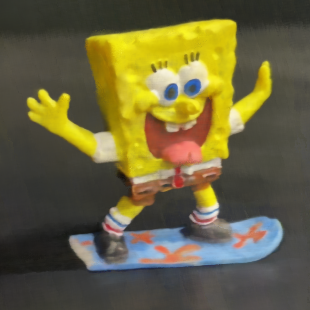
\includegraphics[width=0.3\textwidth]{../images/230717/000.png}}\hfill
    \subfloat[view2 rendered image]{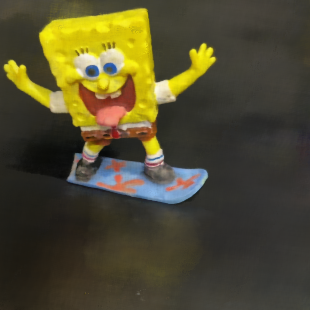
\includegraphics[width=0.3\textwidth]{../images/230717/079.png}}\hfill
    \subfloat[view3 rendered image]{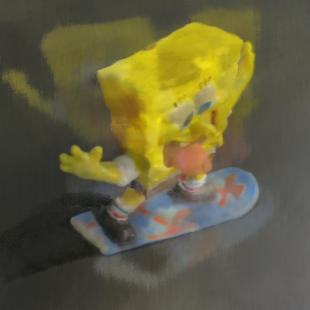
\includegraphics[width=0.3\textwidth]{../images/230717/002.png}}\hfill

    \subfloat[view1 depthmap]{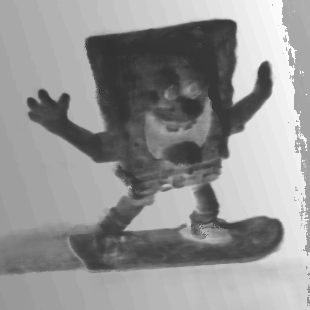
\includegraphics[width=0.3\textwidth]{../images/230717/000_depth.png}}\hfill
    \subfloat[view2 depthmap]{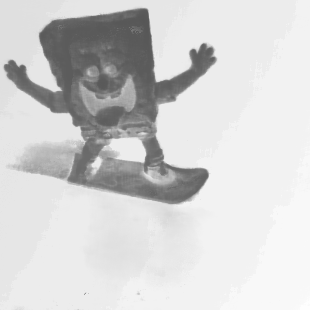
\includegraphics[width=0.3\textwidth]{../images/230717/079_depth.png}}\hfill
    \subfloat[view3 depthmap]{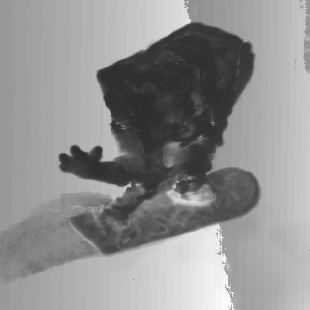
\includegraphics[width=0.3\textwidth]{../images/230717/002_depth.png}}\hfill

    \caption{Results of InfoNeRF with 38 scenes}
    \label{fig:Results}
\end{figure}

추가적으로 camera extrinsic을 잘못 구하였을 가능성이 있기 때문에
hash nerf를 사용해 결과를 얻어본 결과 좋은 성능의 depthmap이 나온것을 확인 가능하였다. 





\section*{Action items in next week}	%% Action items in next week
다음 주에는 
\begin{enumerate}
    \item InfoNeRF 추가학습
    \item point cloud 시각화 
\end{enumerate}
등을 진행하도록 하겠습니다.

\bibliographystyle{IEEEtran} 
\bibliography{refer} 
\end{document}